\section{Používateľská špecifikácia} % 3-4 strany
\subsection{Stručný úvod do problematiky}
\acrfull{mhs} \projectName\ má ľuďom uľahčiť vyhľadávanie a rezerváciu 
ubytovania v rôznych krajinách sveta.
Systém je určený pre dve skupiny používateľov. 
Pre potenciálnych zákazníkov hotelov alebo iných ubytovacích zariadení, 
ktorí si chcú rezervovať najviac vyhovujúce ubytovanie v čo najlacnejšej 
ponuke v ich vybranej lokalite v určitom čase. 
A pre poskytovateľov ubytovania, ktorí dokážu a chcú poskytovať ubytovanie 
a služby s tým spojené. 
\acrshort{mhs} eviduje všetky možné destinácie, v ktorých si vie 
potenciálny zákazník vyberať a porovnávať ubytovacie zariadenia a následne 
zarezervovať vo vybranom čase, ak je ubytovacie zariadenie vtedy voľné. 
Evidenciu destinácií vytvárajú samotní poskytovatelia ubytovancích zariadení, 
pri zadávaní lokalít, kde sa nachádza poskytované ubytovanie. 
Poskytovatelia ubytovania môžu byť fyzické osoby, živnostníci, hotely, 
cestovné kancelárie a rôzne iné spoločnosti, ktoré sa zaoberajú turizmom 
a hotelierstvom. 
Po zaregistrovaní poskytovateľa ubytovania v \acrshort{mhs} a overení 
pravdivosti údajov je mu vytvorený účet v systéme, do ktorého môže vložiť 
svoju ponuku ubytovania a k nemu prezentačné materiály o ubytovaní a informácie 
ako repertoár poskytovaných služieb, cenník, počet voľných miest v rôznych 
časových obdobiach, kontaktné údaje, podmienky a pravidlá ubytovania a 
poprípade zaujímavé tipy na výlety, občerstvenie alebo aktivity. 
Neregistrovaný poskytovateľ nie je schopný vykonať takéto úkony v 
\acrshort{mhs}, kvôli ochrane potenciálneho zákazníka, aby mal istotu, že 
poskytovateľ je skutočná osoba alebo subjekt a ubytovacie zariadenie vôbec 
existuje alebo existuje na danom mieste a vedia mu garantovať všetko, 
čo by bolo v ponuke ubytovania uvádzané a nebol teda zákazník zavádzaný. 
Potenciálny alebo už aktuálny zákazník registráciou do \acrshort{mhs} vie 
získať možnosť hodnotiť ubytovacie zariadenia ako aj ich poskytovateľov a 
nimi ponúkané služby a to aj anonymne a taktiež mu \acrshort{mhs} vie uložiť a 
poskytnúť k nahliadnutiu celú históriu rezervácii ubytovaní.
Neregistrovaní zákazníci vedia iba vyhľadávať a prezerať si 
všetky ponuky ubytovania v rôznych krajinách sveta.
Na samotnú rezerváciu ubytovania musí zákazník byť registrovaný a to z dôvodu 
ochrany poskytovateľov ubytovania, aby zákazník bol viazaný na určité pravidlá 
a povinosti pri rezervovaní ubytovania a aby poskytovateľ mal zaručený kontakt so 
zákazníkom, pri vzniknutých komplikáciach z poskytovateľovej strany.
\acrshort{mhs} poskytuje podporu pre automatické zisťovanie rôznych parametrov 
prostredníctvom webových služieb alebo ako \acrfull{api}, ktoré 
zabezpečujú dostupnosť a aktuálnosť údajov v \acrshort{mhs}.
Vďaka \acrshort{mhs} \projectName\ poskytovateľ nemusí mať na spravovanie 
rezervácií vyhradeného zamestnanca alebo skupinu personálu, keďže o veľkú časť 
sa postará už zákazník ako o samotnú rezerváciu izby/zariadenia v jeho 
určenom čase, vyplnenie a kontrolu správnosti údajov a oboznámenie sa so 
službami. Poskytovateľ už musí len zobrať na vedomie zákazníkovú rezerváciu, 
prijať ju alebo ju zamietnuť s relevantným dôvodom a kontaktovať s tým 
zákazníka. Pri prijatí rezervácie musí zabezpečiť personál, ak nejaký má, a 
zabezpečí sľúbené služby a čistotu priestorov pri príchode alebo počas celého 
pobytu zákazníka, podľa vopred dohodnutých podmienok.

\newpage
\subsection{Používateľské požiadavky}
\begin{enumerate}[label=\Alph*]
    \item Funkcionálne požiadavky
    \begin{itemize}
        \item List entries start with the \verb|\item| command.
        \item Individual entries are indicated with a black dot, a so-called bullet.
        \item The text in the entries may be of any length.
    \end{itemize}
    \item Nefunkcionálne požiadavky
    \begin{itemize}
        \item List entries start with the \verb|\item| command.
        \item Individual entries are indicated with a black dot, a so-called bullet.
        \item The text in the entries may be of any length.
    \end{itemize}
    \item Doménové požiadavky
    \begin{itemize}
        \item List entries start with the \verb|\item| command.
        \item Individual entries are indicated with a black dot, a so-called bullet.
        \item The text in the entries may be of any length.
    \end{itemize}
\end{enumerate}

%%%%%%%%%%%%%%%%%%%%%%%%%%%%%%%%%%%%%%%%%%%%%%%%%%%%%%%%%%%%%%%%%%%%%%%%

\section{Systémová špecifikácia}
V diagramoch použite notáciu UML verzie 2.x

\subsection{Diagramy prípadov použitia.}
Nakreslite diagram(y) prípadov použitia pre daný softvérový
systém. Diagram (minimálne jeden, prípadne viacej ak sa to hodí), bude pomocou prípadov
použitia obsahovať celú hlavnú funkcionalitu systému. Každý prípad použitia by mal, v rámci
svojej realizácie, poskytovať svojmu hráčovi (alebo hráčom) niečo hodnotné, nejakú užitočnú
funkcionalitu, nejaký pozorovateľný výsledok alebo zmenu.

\subsection{Use-case tabuľky}
K trom najzložitejším prípadom použitia vytvorte use-case tabuľku, ktorá
bude obsahovať [2b]:
– názov prípadu použitia
– identifikátor - ako identifikátor môžete použiť svoje vlastné číslovanie, ktoré bude
spájať jednotlivé prípady použitia z diagramu prípadov použitia.
– opis prípadu použitia (stručný)
– hráčov
– vstupné podmienky
– inicializácia
– hlavnú postupnosť udalostí
– alternatívnu postupnosť udalostí
– výstupné podmienky
VZOR: tutoriál č.2 – \href{https://uim.fei.stuba.sk/wp-content/uploads/2022/09/CV2-USC_tabulka_TUTORIAL.pdf}{use-case tabuľka}

\subsection{Diagram tried}
Vytvorte jeden detailný dátový model pre celý váš systém, ktorý bude zahŕňať
všetky atribúty, vzťahy, násobnosti a aspoň niektoré metódy. Zobrazte ho ako jeden UML 2.x
diagram tried vo vašej výslednej dokumentácii. Ak je systém príliš komplexný, môžete rozčleniť
diagram na viacero menších diagramov, ktoré budú reprezentovať len príslušný podsystém.

\subsection{Diagramy aktivít a sekvenčné diagramy}
K vybraným netriviálnym prípadom použitia nakreslite
diagramy graficky popisujúce tieto prípady použitia. Nakreslite 2 sekvenčné diagramy a 2
diagramy aktivít.

\subsection{Stavový diagram}
Nakreslite stavový diagram pre vami vyvíjaný systém a v tabuľkách popíšte
jednotlivé stavy a prechody. Môžete vytvoriť aj viacero menších stavových diagramov namiesto
jedného veľkého.

%%%%%%%%%%%%%%%%%%%%%%%%%%%%%%%%%%%%%%%%%%%%%%%%%%%%%%%%%%%%%%%%%%%%%%%%

\section{Akceptačné testy}
Vytvorte testy, na základe ktorých sa rozhodne o tom, či vytvorený systém spĺňa alebo nespĺňa
požiadavky – teda či ho zákazník akceptuje alebo nie. Každý test by mal v tabuľke obsahovať minimálne
tieto časti:
• identifikátor
• prípad použitia, ku ktorému test prislúcha
• cieľ testu (čo overujeme – nanajvýš stručne)
• vstupné podmienky
• výstupné podmienky
• jednotlivé kroky testu
Kroky testu reprezentujú sekvenciu testovania a ku každému kroku prislúcha a je v teste popísaná určitá
akcia (podnet od aktéra) a určitá reakcia systému na tento podnet. Aby bol výsledný systém zákazníkom
akceptovaný, musí splniť všetky testy. Keďže v tomto zadaní systém neprogramujeme ale len
navrhujeme, jednotlivé očakávané reakcie je potrebné si vymyslieť.
Do dokumentácie doplňte aspoň 5 akceptačných testov
• štyri, ktoré súvisia s funkcionálnymi požiadavkami a
• jeden, ktorý overuje nefunkcionálne požiadavky.
PRÍKLAD: \href{https://uim.fei.stuba.sk/wp-content/uploads/2022/10/AkceptacneTestyPriklad.pdf}{AkceptacneTestyPriklad.pdf}

%%%%%%%%%%%%%%%%%%%%%%%%%%%%%%%%%%%%%%%%%%%%%%%%%%%%%%%%%%%%%%%%%%%%%%%%

\section{Projektové plánovanie}
Vytvorte plán tvorby (realizácie) vášho systému.
1. Rozdeľte prácu na aspoň 10 úloh a rozdeľte úlohy pre aspoň 4 ľudí tvoriacich váš tím. Počet si zvoľte
podľa náročnosti témy, ale minimálne musí mať váš tím aspoň 4 členov.
2. Odhadnite časovú náročnosť úloh, naplánujte postupnosť úloh do kalendára.
3. V dokumente v kapitole 4.1 zobrazte Ganttov graf aj s tabuľkou závislostí a postupnosti vykonávania
úloh, s míľnikmi a s WBS (work breakdown schedule).
4. V dokumente v kapitole 4.2. zobrazte sieťový graf pre postupnosti vykonávania úloh.
Na túto úlohu použite vami zvolený systém na projektový manažment (či už offline, lokálny program
alebo ľubovoľný/dostupný online produkt). Zoznam je napr. na:
\url{http://en.wikipedia.org/wiki/Comparison_of_project-management_software}. Úlohou je oboznámiť sa
so systémom na projektový manažment.
Odporúčame: Microsoft Project, Project Libre alebo google: alternatives to ms project

%%%%%%%%%%%%%%%%%%%%%%%%%%%%%%%%%%%%%%%%%%%%%%%%%%%%%%%%%%%%%%%%%%%%%%%%

% \begin{table}[!htbp]
% \caption{Moduly a ich funkcie pri anonymizácii}
% \label{modulyVlastnosti}
% \begin{center}
% \begin{tabular}{p{4cm}|c|c|c|c|c|c|c|c|c|c|c|c|c|c|c}
% & \multicolumn{14}{c}%
% 	 {\textbf{Funkcia}}\\ \hline
% &&&& & &\multicolumn{8}{c}%
% 	 {Modifikácia}\\ 
% \textbf{Modul} &\begin{sideways} zobrazenie hlavičky \end{sideways} &\begin{sideways} blokovanie skriptov \end{sideways} &\begin{sideways} zmena IP \end{sideways} & \begin{sideways} zmena lokalizácie \end{sideways} & \begin{sideways} zmazanie/blokovanie cookies \end{sideways} & \begin{sideways} blokovanie trackerov \end{sideways}  & \begin{sideways} popis \end{sideways} & \begin{sideways}používateľský agent\end{sideways} & \begin{sideways} kódové označenie prehliadača \end{sideways} & \begin{sideways} názov prehliadača \end{sideways} & \begin{sideways} verzia prehliadača \end{sideways} & \begin{sideways} platforma \end{sideways} & \begin{sideways} výrobca prehliadača \end{sideways} & \begin{sideways} označenie výrobcu prehliadača \end{sideways} \\ \hline
% User agent switcher & & & & & &  & X & X & X & X & X & X & X & X  \\ \hline
% Ghostery &  && & & X & X &  &  & & & & & & \\  \hline
% Better privacy && &  & & X &  &  &  & & & & & & \\  \hline
% Anonymox &  && X & X & X &  & X & X & & & & & & \\  \hline
% Modify headers & & &  &  & X &  &  & X &  &  &  & & &  \\  \hline
% Request policy & & &  &  & & X  &  &  &  &  &  & & &   \\  \hline
% Live HTTP headers & X& &  &  & &  &  &  &  &  &  & & &   \\  \hline
% User agent awitcher & & &  &  & &  & X & X &  &  &  & & &   \\  \hline
% Header hacker & & &  &  & &  & X & X & X & X & X & X & X & X    \\  \hline
% Mod header & & &  &  & &  & X & X & X & X & X & X & X & X    \\  \hline
% Script no & &X &  &  & &  &  &  &  &  &  &  &  &     \\  \hline
% No script & &X &  &  & &  &  &  &  &  &  &  &  &     \\  \hline
% Proxify it & & &X  & X & &  &  &  &  &  &  &  &  &     \\  \hline
% I'm not here & & &  & X & &  &  &  &  &  &  &  &  &     \\  \hline
% Get edition & &X &X &X &X&X &  &  &  &  &  &  &  &     \\  \hline
% Anonymous browsing toolbar & & & X & X & &  &  &  &  &  &  &  &  &     \\  \hline
% Easy hide your IP and surf & & & X & X& &  &  & X & X & X & X &  &  &     \\  \hline
% \end{tabular}
% \end{center}
% \end{table}

% \begin{figure}[!htbp]
%   \centering
%   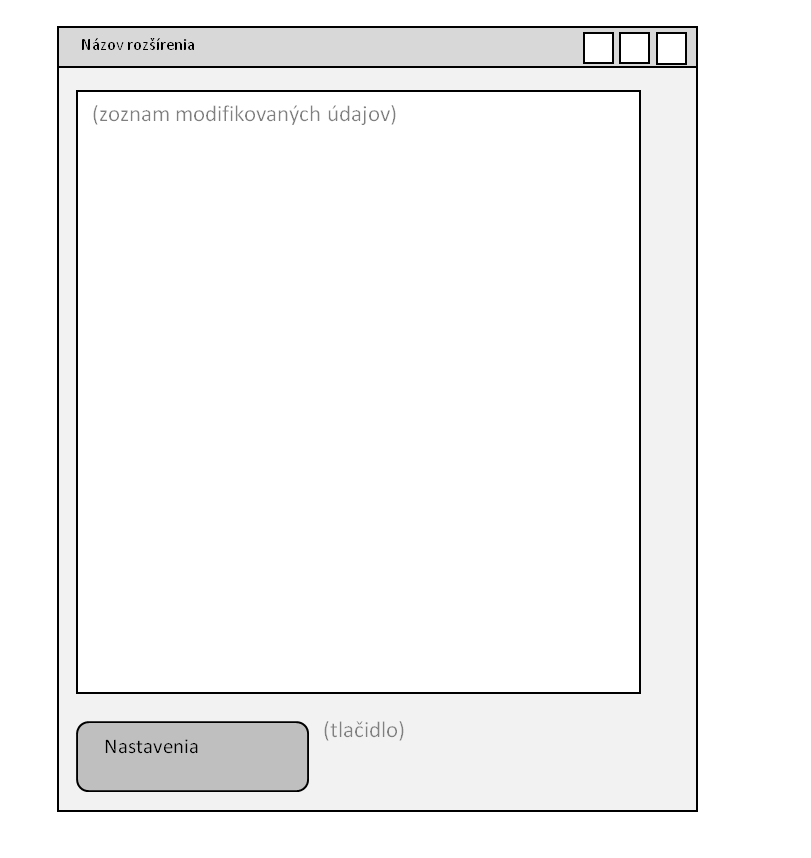
\includegraphics[width=8cm]{img/vzhlad.png}
%   \caption{Predpokladaný vzhľad rozšírenia.}
%   \label{vzhladobr}
% \end{figure}	 

% \begin{algorithm}
% \scriptsize
% \begin{algorithmic}
%  \STATE <text>
%  \IF{<condition>} \STATE {<text>} \ELSE \STATE{<text>} \ENDIF
%  \IF{<condition>} \STATE {<text>} \ELSIF{<condition>} \STATE{<text>} \ENDIF
%  \FOR{<condition>} \STATE {<text>} \ENDFOR
%  \FOR{<condition> \TO <condition> } \STATE {<text>} \ENDFOR
%  \FORALL{<condition>} \STATE{<text>} \ENDFOR
%  \WHILE{<condition>} \STATE{<text>} \ENDWHILE
%  \REPEAT \STATE{<text>} \UNTIL{<condition>}
%  \LOOP \STATE{<text>} \ENDLOOP
%  \REQUIRE <text>
%  \ENSURE <text>
%  \RETURN <text>
%  \PRINT <text>
%  \COMMENT{<text>}
%  \AND, \OR, \XOR, \NOT, \TO, \TRUE, \FALSE
% \end{algorithmic}
% \caption{Ukážka príkazov pre algorithmic}  
% \label{alg:preview}  
% \end{algorithm}

% \begin{lstlisting}[
%   caption={Ukážka algoritmu},
%   label={lst:main-c},
%   language=c
% ]
% /* Hello World program */

% #include<stdio.h>

% struct cpu_info {
%     long unsigned utime, ntime, stime, itime;
%     long unsigned iowtime, irqtime, sirqtime;
% };

% main()
% {
%     printf("Hello World");
% }
% \end{lstlisting}